\documentclass{ximera}
\newcommand{\RR}{\mathbb R}
\renewcommand{\d}{\,d}
\newcommand{\dd}[2][]{\frac{d #1}{d #2}}
\renewcommand{\l}{\ell}
\newcommand{\ddx}{\frac{d}{dx}}
\newcommand{\dfn}{\textbf}
\newcommand{\eval}[1]{\bigg[ #1 \bigg]}

\author{Tom Dinitz and Nela Lakos}
\license{Creative Commons 3.0 By-NC}
\title{Formula Sheet}

\begin{document}
\begin{abstract}
Formula Sheet
\end{abstract}
\maketitle

PERIMETERS AND AREAS

\begin{image}
  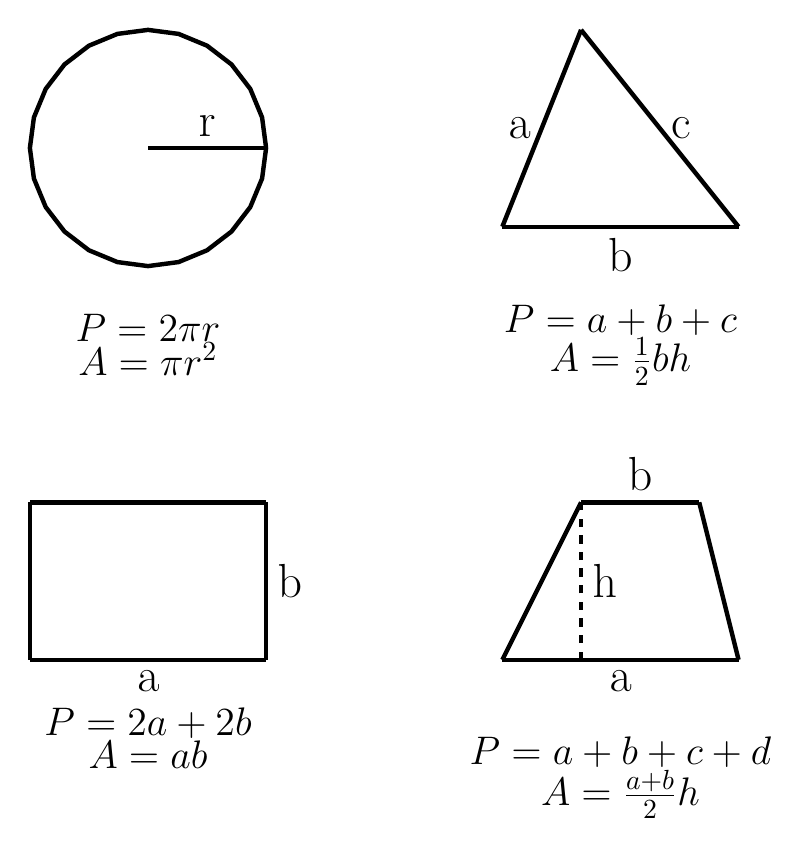
\begin{tikzpicture}
    %draw (0,0) -- (0,6);
    %\draw (0,0) -- (12,0);
    %\draw (6,0) -- (6,12);
    %\draw (0,6) -- (12,6);
    %\draw (12,0) -- (12,12);
    %\draw (0,12) -- (12,12);

   %CIRCLE
    \draw [ultra thick,domain=0:360] plot ({1.5*cos(\x)+3}, {1.5*sin(\x)+9.5});
    \draw [ultra thick](3,9.5) -- (4.5,9.5) node[pos=0.5, above]{\LARGE r};
    \node at (3,7) [align=center] {\Large $P=2\pi r$\\ \Large $A=\pi r^2$};

    %\draw [penColor,ultra thick,domain=270:360] plot ({2*cos(\x)+8}, {2*sin(\x)+11});
    %\draw [penColor,ultra thick,domain=0:90] plot ({2*cos(\x)+2}, {2*sin(\x)+3});
    %\draw [penColor,ultra thick,domain=180:90] plot ({2*cos(\x)+10}, {2*sin(\x)+3});
 
    %TRIANGLE    
	\draw [ultra thick] (7.5,8.5) -- (10.5,8.5) node[pos=0.5, below]{\LARGE b};
 	\draw [ultra thick] (7.5,8.5) -- (8.5,11) node[pos=0.5, left]{\LARGE a};
 	\draw [ultra thick]  (8.5,11) -- (10.5,8.5) node[pos=0.5, right]{\LARGE c};
 	\node at (9,7) [align=center] {\Large $P=a+b+c$\\ \Large $A=\frac{1}{2}bh$};

    %RECTANGLE
	\draw [ultra thick] (1.5,3) -- (4.5,3) node[pos=0.5, below]{\LARGE a};
 	\draw [ultra thick] (4.5,3) -- (4.5,5) node[pos=0.5, right]{\LARGE b};
 	\draw[ultra thick]  (4.5,5) -- (1.5,5);
	\draw [ultra thick] (1.5,5) -- (1.5,3);
	
	\node at (3,2) [align=center] {\Large $P=2a+2b$\\ \Large $A=ab$};
	
	%TRAPEZOID
	\draw [ultra thick] (7.5,3) -- (10.5,3) node[pos=0.5, below]{\LARGE a};
 	\draw [ultra thick] (10.5,3) -- (10,5) ;
 	\draw[ultra thick]  (10,5) -- (8.5,5)node[pos=0.5, above]{\LARGE b};
	\draw [ultra thick] (8.5,5) -- (7.5,3);
	\draw[dashed,ultra thick]  (8.5,3) -- (8.5,5) node[pos=0.5,right] {\LARGE h};
	
	\node at (9,1.5) [align=center] {\Large $P=a+b+c+d$\\ \Large $A=\frac{a+b}{2}h$};
	
 \end{tikzpicture}
 \end{image}
 
 VOLUMES AND SURFACE AREAS

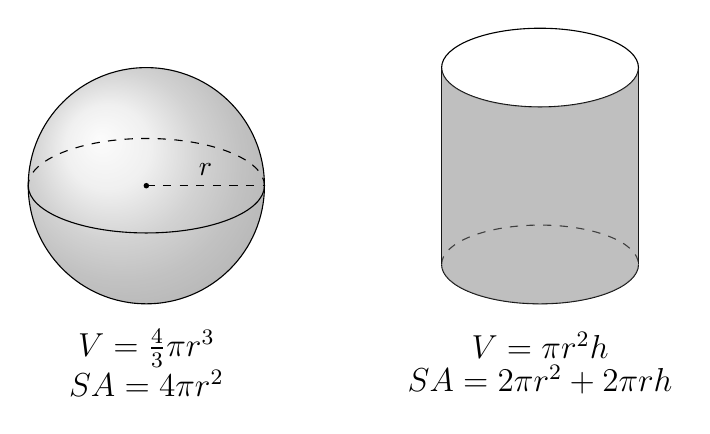
\begin{tikzpicture}
%SPHERE
  \shade[ball color = gray!40, opacity = 0.4] (2,0) circle (1.5cm);
  %\node at (0,0) [align=center]{a};
  \draw (2,0) circle (1.5cm);
  \draw (.5,0) arc (180:360:1.5 and 0.6);
  \draw[dashed] (3.5,0) arc (0:180:1.5 and 0.6);
  \fill[fill=black] (2,0) circle (1pt);
  \draw[dashed] (2,0 ) -- node[above]{$r$} (3.5,0);
  
  \node at (2,-2.25) [align=center] {\large $V=\frac{4}{3}\pi r^3$\\ \large $SA=4\pi r^2$};
  
  %CYLINDER
\draw (7,1.5) ellipse (1.25 and 0.5);
\draw (5.75,1.5) -- (5.75,-1);
\draw (5.75,-1) arc (180:360:1.25 and 0.5);
\draw [dashed] (5.75,-1) arc (180:360:1.25 and -0.5);
\draw (8.25,1.5) -- (8.25,-1);  
\fill [gray,opacity=0.5] (5.75,1.5) -- (5.75,-1) arc (180:360:1.25 and 0.5) -- (8.25,1.5) arc (0:180:1.25 and -0.5);
\node at (7,-2.25) [align=center] {\large $V=\pi r^2h$\\ \large $SA=2\pi r^2+2\pi rh$};
\end{tikzpicture}

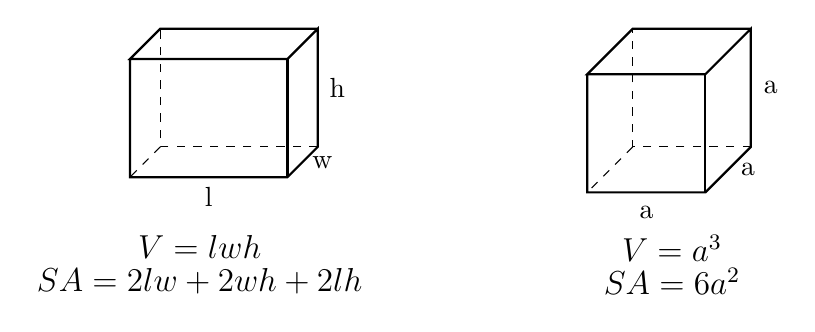
\begin{tikzpicture}
\pgfmathsetmacro{\xr}{3.5}
\pgfmathsetmacro{\xl}{1.5}
\pgfmathsetmacro{\yt}{0}
\pgfmathsetmacro{\yb}{-1.5}
\pgfmathsetmacro{\zi}{0}
\pgfmathsetmacro{\zo}{1}
  \draw[thick](\xr,\yt,0)--(\xl,\yt,\zi)--(\xl,\yt,\zo)--(\xr,\yt,\zo)--(\xr,\yt,\zi)--(\xr,\yb,\zi)--(\xr,\yb,\zo)--(\xl,\yb,\zo)--(\xl,\yt,\zo);
  \draw[thick](\xr,\yt,\zo)--(\xr,\yb,\zo);
  \draw[dashed](\xr,\yb,\zi)--(\xl,\yb,\zi)--(\xl,\yt,\zi);
  \draw[dashed](\xl,\yb,\zi)--(\xl,\yb,\zo);
  \draw(\xr+.25,\yt*.5+\yb*.5,\zi) node{h};
  \draw(\xr+.25,\yb,\zi*.5+\zo*.5) node{w};
  \draw(\xl*.5+\xr*.5,\yb-.25,\zo) node{l};
\node at (2,-3) [align=center] {\large $V=lwh$\\ \large $SA=2lw+2wh+2lh$};  
  
  \pgfmathsetmacro{\cxr}{9}
\pgfmathsetmacro{\cxl}{7.5}
\pgfmathsetmacro{\cyt}{0}
\pgfmathsetmacro{\cyb}{-1.5}
\pgfmathsetmacro{\czi}{0}
\pgfmathsetmacro{\czo}{1.5}
  \draw[thick](\cxr,\cyt,0)--(\cxl,\cyt,\czi)--(\cxl,\cyt,\czo)--(\cxr,\cyt,\czo)--(\cxr,\cyt,\czi)--(\cxr,\cyb,\czi)--(\cxr,\cyb,\czo)--(\cxl,\cyb,\czo)--(\cxl,\cyt,\czo);
  \draw[thick](\cxr,\cyt,\czo)--(\cxr,\cyb,\czo);
  \draw[dashed](\cxr,\cyb,\czi)--(\cxl,\cyb,\czi)--(\cxl,\cyt,\czi);
  \draw[dashed](\cxl,\cyb,\czi)--(\cxl,\cyb,\czo);
  \draw(\cxr+.25,\cyt*.5+\cyb*.5,\czi) node{a};
  \draw(\cxr+.25,\cyb,\czi*.5+\czo*.5) node{a};
  \draw(\cxl*.5+\cxr*.5,\cyb-.25,\czo) node{a};
\node at (8,-3) [align=center] {\large $V=a^3$\\ \large $SA=6a^2$};  
  
\end{tikzpicture}

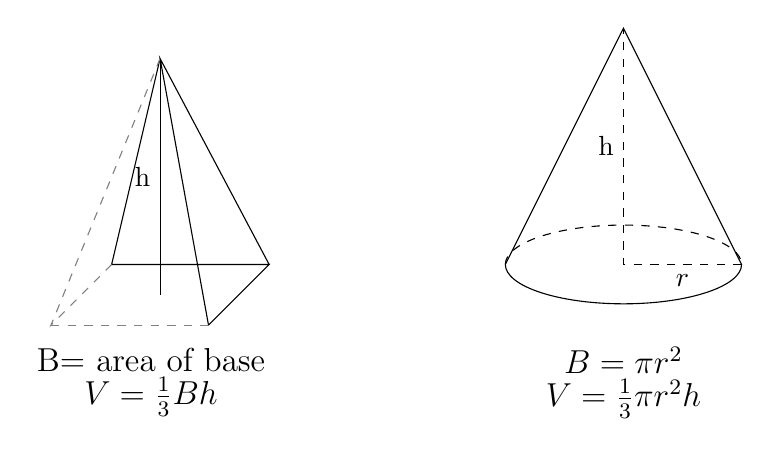
\begin{tikzpicture}
    \draw (1,3,1) -- (0,0,0) -- (2,0,0) -- (2,0,2) -- (1,3,1) 
      -- (2,0,0);
    \draw[color=gray, style=dashed] (1,3,1) -- (0,0,2) 
      -- (0,0,0);
    \draw[color=gray, style=dashed] (0,0,2) -- (2,0,2);
    \draw (4.6,-.2,2);
    \draw(1,3,1) -- node[left] {h} (1,0,1);

 \node at (0.5,-1.5) [align=center] {\large B= area of base\\ \large $V=\frac{1}{3}Bh$}; 
 
\draw 
  (5,0) arc (180:360:1.5 and .5) -- (6.5,3) -- cycle;
\draw[dashed]
  (5,0) arc (180:0:1.5 and .5);
\draw[dashed]
  (8,0) -- node[below] {$r$} (6.5,0) -- node[left] {h} (6.5,3) ;
  \node at (6.5,-1.5) [align=center] {\large $B= \pi r^2$\\ \large $V=\frac{1}{3}\pi r^2h$}; 
  
\end{tikzpicture}


\end{document}